%!TEX root = ../main.tex

\section{Introduction}

\begin{frame}
\frametitle{Recent developments in Lightning solvers}
\begin{figure}
	\captionsetup{position=top}
	\centering
	\subcaptionbox*{Laplace (old)}{
	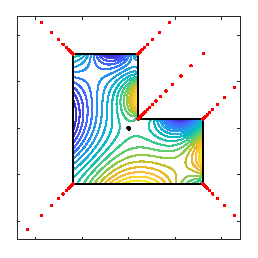
\includegraphics[width=0.3\linewidth]{Figures/intro1}}
	\subcaptionbox*{Stokes (new)}{
	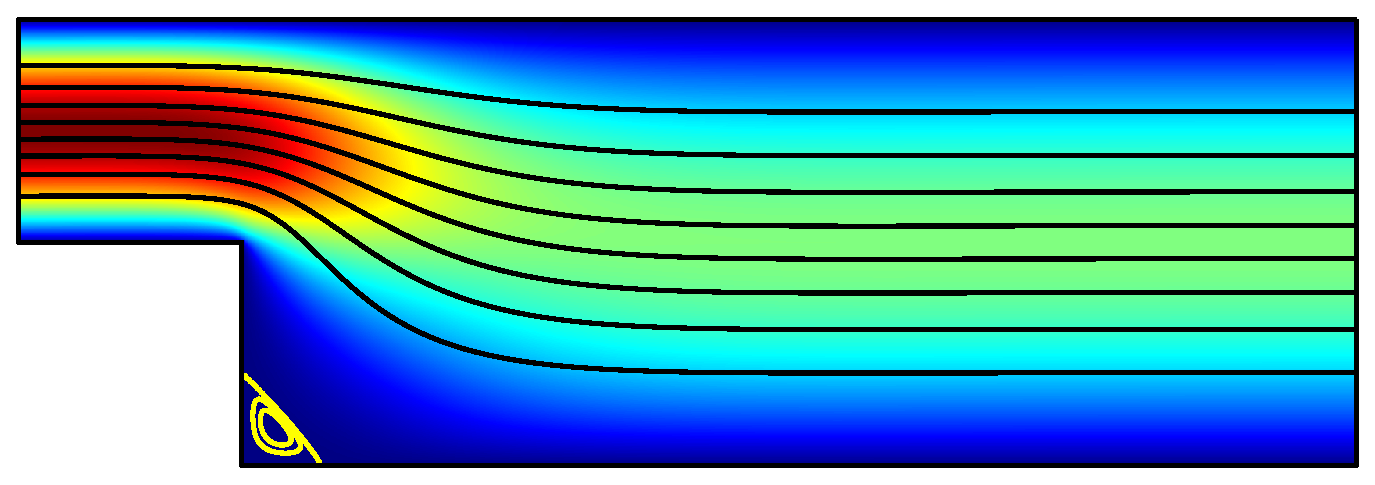
\includegraphics[width=0.66\linewidth]{Figures/intro2}}
	\vfill
	\subcaptionbox*{$-\infty\xleftarrow{\hspace*{0.3\linewidth}}$ Laplace (new) $\xrightarrow{\hspace*{0.3\linewidth}}\infty$}{
	
\includegraphics[width=\linewidth]{Figures/intro3}}
\end{figure}
\end{frame}